\section{Experimental Data and Image Processing Workflow}

\subsection{Workflow Overview}

Figure~\ref{fig:surrogate-data-flow} illustrates the overall data flow of the surrogate modeling workflow used in this thesis, organized into four swimlanes.
Raw inputs (high-speed Mie videos, calibration configurations, and test metadata) first undergo CUDA-accelerated image processing to generate 1D features and boundary points; based on this, binary-thresholded (BW) and CDF-based penetration trajectories along with other geometric metrics are obtained.
These observables are expanded into synthetic trajectories via non-parametric curve fitting and are used to drive a three-stage neural network training: Stage~1 (MSE), Stage~2 (NLL), and Stage~3 (Raw + KD, knowledge distillation).
The ultimately trained model is deployed in a wall impingement screening application, which outputs impingement probabilities and visualization animations in combination with piston geometry and physical parameters.
Table~\ref{tab:workflow} summarizes these same stages in textual form.
This chapter focuses on the first two swimlanes of Figure~\ref{fig:surrogate-data-flow}: how the Optical Spray Combustion Chamber (OSCC) video data undergoes calibration, preprocessing, registration, and conversion into plume-resolved geometric observables.
The construction of trajectory targets, surrogate modeling training, and probabilistic screening are deferred to the next chapter.

Raw per-frame boundary extraction alone cannot supply the surrogate of Chapter~4 with what it needs: a fixed-cardinality, censoring-flagged, plume-resolved time series that is comparable across nozzles with different hole counts and frame rates.
This chapter therefore treats image processing as an auditable methodological stage rather than an ancillary preprocessing step; its five methodological elements (listed below) are what convert a discrete, event-by-event observation table into that structured target.
Existing spray-image analyses often report penetration, cone angle, or boundary descriptors for individual operating conditions.
In contrast, the surrogate models in this thesis require consistent, plume-resolved, and censoring-aware time-series targets across many nozzle geometries and operating conditions.
This chapter therefore addresses the target-construction gap between raw optical spray recordings and machine-learning-ready observables.

These tasks are performed based on data from the Wärtsilä OSCC.
The raw materials are terabytes of room-temperature, non-reacting, top-view Mie scattering recordings, acquired across multiple operating conditions and nozzle geometries under a fixed camera setup.
The pipeline first manually calibrates the nozzle geometry, then generates plume-resolved observables via CUDA-accelerated preprocessing, polar registration, and plume strip extraction,
and constructs penetration targets through reduced-order fitting, which are subsequently passed to the three-stage MLP surrogate described in Chapter~4.
At the implementation level, this image-processing stage is built as a four-lane overlapped pipeline---disk prefetch, GPU compute, CPU feature extraction, and asynchronous output running concurrently---governed by a resumable checkpoint contract, so that the multi-terabyte archive is reprocessed end-to-end on a single workstation GPU rather than through serial frame-by-frame processing (Section~\ref{subsec:concurrency-architecture}).

\smallskip\noindent\textbf{Contributions of this chapter.} This chapter contributes five reusable methodological elements to the image-to-observable pipeline:
\begin{enumerate}
  \item a log-ratio (homomorphic) foreground estimator that treats glare and non-uniform illumination as multiplicative effects and removes them as additive offsets in log space (Section~\ref{subsec:background-normalization});
  \item a rank-1 separable Sobel edge-enhancement stage kept entirely on the GPU as two one-dimensional passes (Section~\ref{subsec:edge-enhancement});
  \item an FFT harmonic-phase alignment that converts the known multi-hole count into an automatic, per-recording plume registration rule rather than a hand-set reference angle (Section~\ref{subsec:plume-registration});
  \item a cumulative-distribution (CDF) penetration front that is robust to fragmented leading-edge pixels while remaining consistent with standard diesel-spray penetration conventions (Section~\ref{subsec:penetration-measurement});
  \item a four-lane overlapped GPU pipeline with a resumable checkpoint contract that reprocesses the multi-terabyte archive end-to-end on a single workstation GPU (Section~\ref{subsec:concurrency-architecture}).
\end{enumerate}

\begin{figure}[t]
\centering

\includegraphics[width=\linewidth]{surrogate_modelling_data_flow.png}
\caption{Overview of the surrogate modeling data flow. The four swimlanes correspond to raw inputs, image processing, data augmentation and deep learning, and model deployment; arrows denote key data transfer and training connections (Median Filtering, Warm Start, Warm Start + Distillation, Supervised Fine-Tuning).}
\label{fig:surrogate-data-flow}
\end{figure}

\begin{table}[t]
\centering
\begin{tabular}{|L{0.21\linewidth}|L{0.26\linewidth}|L{0.33\linewidth}|}
\hline
Stage & Primary Function & Primary Output \\
\hline
Manual Nozzle Calibration & Fix nozzle center, radii, and angular reference & One geometric anchor per recording set \\
\hline
Batch Video Processing \& Plume Extraction & Batch preprocessing, plume-wise feature extraction, and boundary export & Plume-resolved penetration trajectories, binary geometric metrics, and boundary CSVs \\
\hline
Trajectory Cleaning \& Reduced-Order Fitting & Cleaning, temporal alignment, and censoring-aware target construction & Cleaned trajectories, fitting parameters, and fit plots \\
\hline
Stage~1 MSE Baseline & Deterministic representative trajectory training & Training logs, scaler states, \codepath{best\_model\_stage1.pt}, and loss curves \\
\hline
Stage~2 NLL Extension & Learn heteroscedastic mean and variance on the fully filtered dataset & Training logs, scaler states, and teacher checkpoint \codepath{best\_model\_stage2.pt} \\
\hline
Stage~3 Distillation Refinement & Interval-dependent raw CDF distillation and early-time refinement & Run logs, \codepath{best\_model\_refinement.pt}, and ablation summaries \\
\hline
Prototype Probabilistic Screening & Project predicted penetration distributions onto simplified engine geometries to assess near-wall risks & Frame-wise $P_{\mathrm{hit}}(t)$, cumulative $E$, and visualization animations \\
\hline
\end{tabular}
\caption{Implemented workflow documented in this thesis.}
\label{tab:workflow}
\end{table}

\subsection{Experimental Datasets}

The input data originate from a pressurized OSCC operated at the Wärtsilä test facility.
A total of nine nozzles were tested: eight prototype nozzles (Nozzle1--Nozzle8) recorded between October and November 2024,
and one reference injector (Nozzle0) recorded in June 2022.
Table~\ref{tab:nozzle-overview} summarizes the geometry of each nozzle and the range of operating conditions covered,
and Figure~\ref{fig:nozzle-geometry} visualizes the geometric design space spanned by these nozzles.

\begin{table}[t]
\centering
\footnotesize
\setlength{\tabcolsep}{4pt}
\renewcommand{\arraystretch}{1.1}
\begin{tabular}{@{}lcccccc@{}}
\toprule
Nozzle & $d_n$ (mm) & $N$ & $\theta_{\mathrm{umb}}$ (°) & FPS & $P_{\mathrm{inj}}$ (bar) & $t_{\mathrm{inj}}$ (\si{\micro s}) \\
\midrule
Nozzle1 & 0.384 & 10 & 140 & 25{,}000 & 2000          & 560--779   \\
Nozzle2 & 0.375 & 10 & 140 & 25{,}000 & 1400--2000    & 500--917   \\
Nozzle3 & 0.365 & 10 & 140 & 25{,}000 & 2000          & 580--764   \\
Nozzle4 & 0.355 & 10 & 140 & 25{,}000 & 2000          & 558--745   \\
Nozzle5 & 0.348 & 11 & 140 & 25{,}000 & 2000          & 570--763   \\
Nozzle6 & 0.333 & 12 & 140 & 25{,}000 & 2000          & 609--881   \\
Nozzle7 & 0.365 & 12 & 164 & 25{,}000 & 2000          & 580--764   \\
Nozzle8 & 0.365 & 10 & 130 & 25{,}000 & 2000          & 580--764   \\
Nozzle0 & 0.384 & 10 & 140 & 34{,}000 & 1400--2200    & 340--1200  \\
\bottomrule
\end{tabular}
\caption{Nozzle geometries and operating condition ranges. $d_n$: hole diameter; $N$: number of holes; $\theta_{\mathrm{umb}}$: umbrella angle; FPS: recording frame rate; $P_{\mathrm{inj}}$: injection pressure; $t_{\mathrm{inj}}$: commanded injection duration. For Nozzle1--8, the chamber-pressure levels 4.42, 8.84, and 13.26\,bar correspond to logged ambient gas densities of \SI{5}{kg/m^3}, \SI{10}{kg/m^3}, and \SI{15}{kg/m^3}; Nozzle0 records chamber pressure from 5 to 35\,bar. The control back pressure for Nozzle0 is 1\,bar or 4\,bar; Nozzle1--8 did not vary the control back pressure independently.}
\label{tab:nozzle-overview}
\end{table}

\begin{figure}[t]
\centering
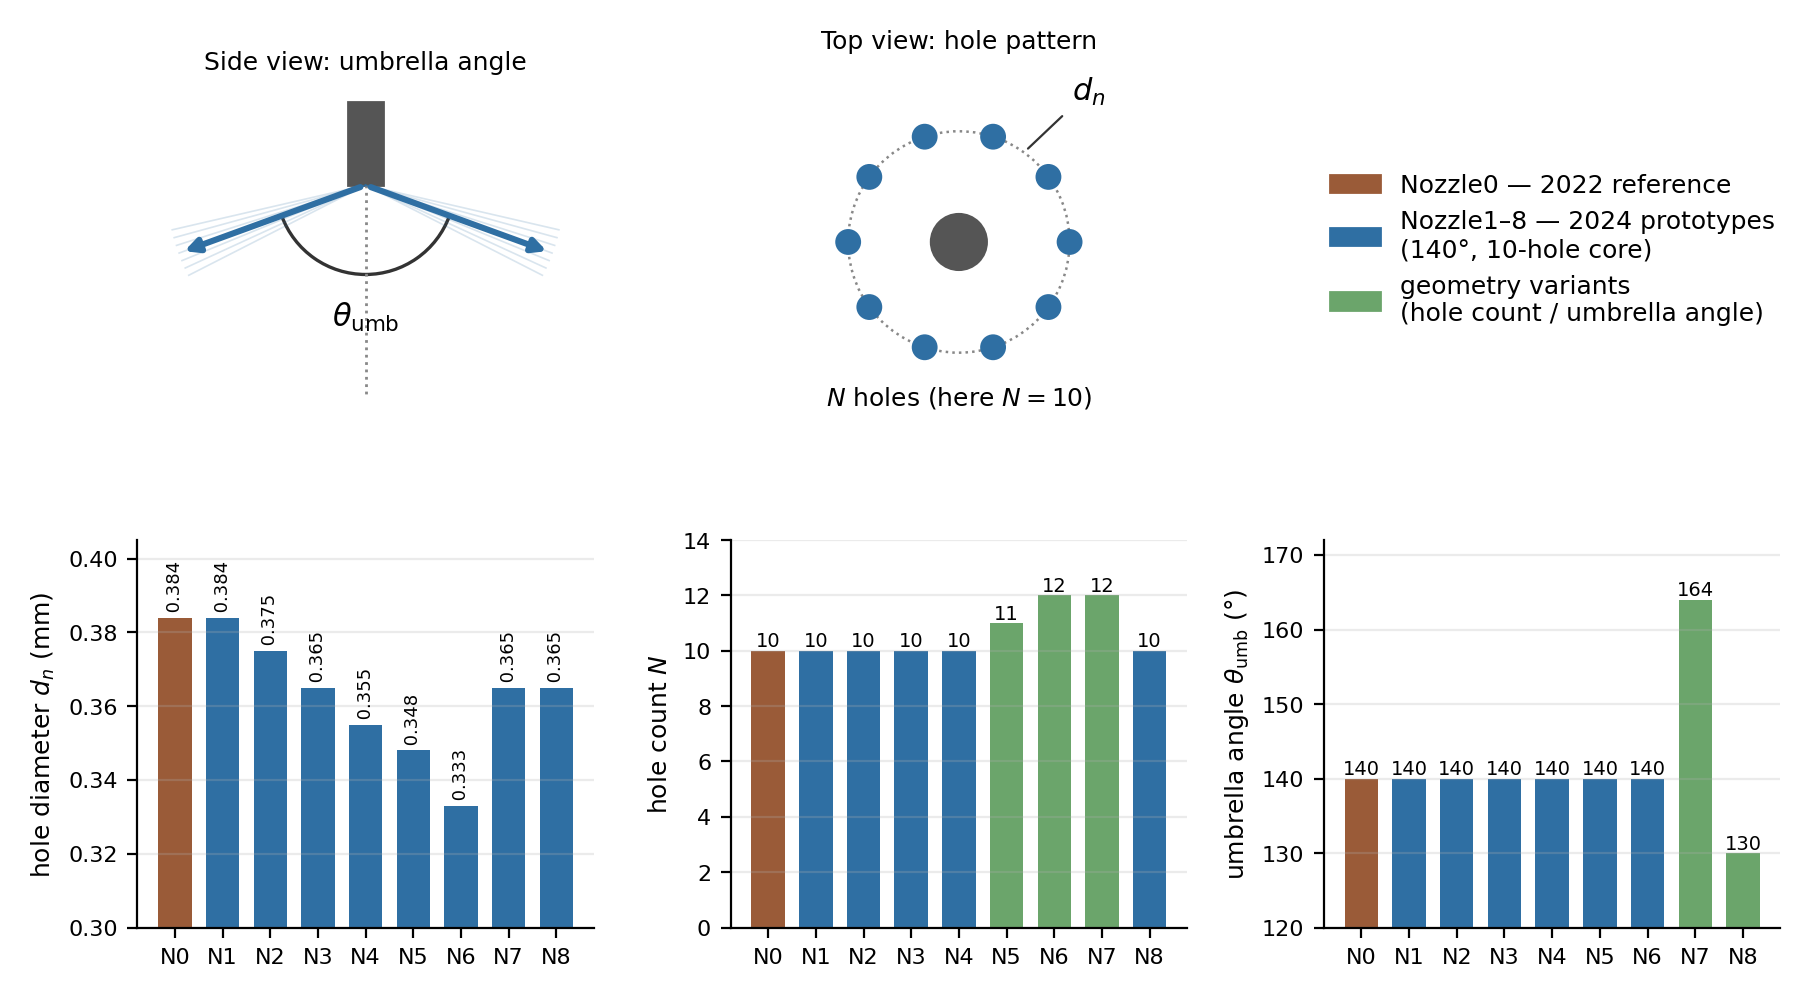
\includegraphics[width=0.95\linewidth]{images/nozzle_geometry_overview.png}
\caption{Geometric design space of the nine nozzles in Table~\ref{tab:nozzle-overview}. Top: schematic definitions of the umbrella angle $\theta_{\mathrm{umb}}$ (side view) and of the hole pattern with hole count $N$ and hole diameter $d_n$ (top view). Bottom: per-nozzle values. Nozzle0 is the 2022 reference injector; Nozzle5--7 vary the hole count and Nozzle7/8 vary the umbrella angle around the 140°, 10-hole core design shared by the remaining prototypes.}
\label{fig:nozzle-geometry}
\end{figure}

Across these nine nozzles, the injection pressure ranges from 1,400 to 2,200\,bar,
the commanded injection duration from 340 to 1,200\,\si{\micro s},
and the chamber pressure from 4.42 to 35\,bar.
Each operating condition subfolder typically contains five repeated recordings,
and each recording is cropped to approximately 100 frames to limit GPU memory footprint.
At the camera frame rates of 25{,}000 and 34{,}000\,FPS used in this study, 100 frames define a physical time window of 4.0\,ms and 2.94\,ms respectively, which is sufficient to capture the pilot injection and its early relaxation tail.
The processed archive totals 266 test condition subfolders and 2{,}992 recording files
(one CSV per \texttt{.cine}); the cropped working archive occupies tens of GB,
while the full uncropped recordings constitute terabytes of raw input.

\subsection{Manual Calibration of Nozzle Geometry}\label{subsec:nozzle-calibration}

Manual calibration fixes the nozzle center, calibration radius, and angular reference used by the subsequent batch processing.
The operator selects visible points on a circular nozzle feature in a representative frame. Mathematically, these selected nozzle edge points $(x_i,y_i)$ are fitted with an algebraic circle model:
\[
x_i^2+y_i^2 + D x_i + E y_i + F = 0,
\]
which is solved via least squares using standard linear solvers (e.g., \texttt{np.linalg.lstsq}) \cite{Pratt1987CircleFit,Taubin1991CircleFit}. The recovered circle parameters are:
\[
c_x=-\frac{D}{2}, \qquad c_y=-\frac{E}{2}, \qquad r=\sqrt{c_x^2+c_y^2-F},
\]
where $(c_x, c_y)$ is the nozzle center and $r$ is the fitted radius. The same fit estimates an average angular offset based on the deviation of the selected edge points from an ideal equally spaced set.
This ideal spacing is used as a nominal injector-geometry reference for anchoring plume-wise coordinates; it does not assert that the observed liquid-phase Mie envelopes remain symmetric or equally spaced after injection.

The calibration values are saved to a configuration file, after which the batch pipeline can process the entire folder without manual recentering. The minimal \texttt{config.json} schema is \{\texttt{plumes}, \texttt{centre\_x}, \texttt{centre\_y}, \texttt{inner\_radius}, \texttt{outer\_radius}\}; the two radii jointly define the annular processing mask, the local orifice origins, and the downstream strip geometry.

The pixel-to-millimeter scale is not obtained through full camera intrinsic calibration, but is back-calculated from the known physical scale of the outer ring:
\[
s_{\mathrm{mm/px}}=\frac{90.0}{r_{\mathrm{outer,px}}},
\]
where $r_{\mathrm{outer,px}}$ is the \texttt{outer\_radius} saved in the configuration file.

The optical path (lens focal length, working distance, and sensor alignment) was configured by the experimental team following standard high-speed imaging practice for the vessel geometry used in this campaign; no formal lens-distortion characterization (e.g.\ a checkerboard intrinsic calibration) was performed or is available for this archive. Because the axial measurement region of interest ($<\SI{90}{mm}$) is small relative to the camera-to-plume working distance, the resulting out-of-plane parallax from the 3D cone expansion of the spray is expected to be a second-order effect relative to the fixed pixel-to-millimeter scale calibrated above; quantitative validation of this assumption is deferred to the downstream LONO consistency checks of Chapter~5.

\begin{figure}[t]
\centering
\begin{minipage}{0.47\linewidth}
\centering

\includegraphics[width=\linewidth]{GUI_calibration_interface.png}\\
(a) Point selection
\end{minipage}
\hfill
\begin{minipage}{0.47\linewidth}
\centering

\includegraphics[width=\linewidth]{GUI_calibration_result.png}\\
(b) Calibration overlay
\end{minipage}
\caption{Nozzle geometry calibration tool. (a) The operator marks visible nozzle-edge points on a representative frame for the algebraic circle fit; (b) the fitted center, plume guide lines, and annular processing mask are overlaid on the recorded spray pattern to verify the geometric anchor before batch processing.}
\label{fig:gui-calibration-workflow}
\end{figure}

This design suits the current dataset because the camera and injector geometries remain fixed within a single recording, and several artifacts concentric with the nozzle in the background can serve as auxiliary references.
Calibrating only once and reusing the same center for all frames avoids inter-frame jitter during downstream plume angle analysis. This one-time calibration is deliberately kept as a user-visible operation rather than fully automated: because camera and injector geometry are fixed for the duration of a recording campaign, a single manually verified calibration is reused across the whole batch, and keeping this step user-visible lets an operator catch a misidentified nozzle center before it silently propagates through thousands of downstream recordings.

\subsection{Batch Video Processing and Plume Extraction}

\begin{figure}[t]
\centering

\includegraphics[width=1\linewidth]{Multi-Hole Top-View Mie Scattering Video Processing Pipeline.png}
\caption{Overview of the multi-hole top-view Mie scattering processing pipeline, from raw \texttt{.cine} recordings, through calibration, CUDA-accelerated preprocessing, plume registration, and penetration extraction, to CSV export.}
\label{fig:pipeline-overview}
\end{figure}

For each recording, the processing chain answers five practical measurement questions, each taken up by a dedicated subsection below: where the nozzle center is (Section~\ref{subsec:nozzle-calibration}), where each plume direction lies (Section~\ref{subsec:plume-registration}), how each plume can be represented in a common local coordinate system (Section~\ref{subsec:binarization-repair} and the affine remapping that precedes it), how far the liquid-phase front has penetrated (Section~\ref{subsec:penetration-measurement}), and which boundary descriptors can be extracted consistently (Section~\ref{subsec:boundary-features}).

For each \texttt{.cine} recording, the processing workflow loads the video into the current array backend, reuses the annular mask for the entire folder, applies the multi-hole preprocessing and postprocessing steps, extracts plume-wise penetration curves, computes boundary-based geometric metrics, and exports synchronized CSV and metadata files.
The most computationally expensive parts of this chain are kept strictly local to the backend: when CuPy is available, convolutions, angular binning, remapping, thresholding, connected component cleaning, and morphological operations are all executed along the CUDA path until the final tabular export.

This implementation choice stems from practical limitations in early internal workflows. The legacy pipeline relied on frame-by-frame MATLAB processing and lacked effective batch parallelism: processing $\sim$50\,GB of videos typically took around a day and was prone to crashing.
Therefore, migrating heavy image operations to a batch CUDA-oriented pipeline is considered a methodological design in this thesis rather than merely a software optimization. All algorithmic stages described in the following subsections run inside this batch pipeline; the concurrency design that lets them execute end-to-end over the full archive on a single GPU---a four-lane overlapped execution model governed by a resumable checkpoint---is detailed in Section~\ref{subsec:concurrency-architecture}, after the individual operations it schedules have been introduced.

\subsubsection{Background Normalization and Foreground Extraction}\label{subsec:background-normalization}

The first algorithmic contribution in the batch pipeline is a foreground construction stage designed for noisy Mie videos, rather than schemes aimed at ideal binary images.
The goal is to estimate a stable relative foreground contrast under non-uniform illumination before any geometric measurement is made.
In the log-ratio foreground extraction step, the raw frame \(V_t(x,y)\) is mapped to
\[
L_t(x,y)=\log(V_t(x,y)+\varepsilon),
\qquad
L_{\mathrm{bkg}}(x,y)=\operatorname{median}_{t<t_{\mathrm{SOI}}} L_t(x,y),
\]
followed by a log-ratio reconstruction:
\[
R_t(x,y)=\exp\!\left(L_t(x,y)-L_{\mathrm{bkg}}(x,y)\right)-1
=\frac{V_t(x,y)-B(x,y)}{B(x,y)+\varepsilon}.
\]
The next step multiplies \(R_t\) by an intensity gate \(M_t(x,y)=\mathbf{1}[V_t(x,y)>\alpha B(x,y)]\), subtracts the pre-injection baseline, and applies a soft threshold
\[
F_t(x,y)=\max\!\left(M_t(x,y)R_t(x,y)-R_0(x,y)-\tau,\,0\right),
\]
where \(\varepsilon\) is a small constant to prevent log-zero, \(t_{\mathrm{SOI}}\) is the start of injection, \(B(x,y)=\exp(L_{\mathrm{bkg}}(x,y))-\varepsilon\) is the linear-scale background, \(\alpha\) is the contrast multiplier for the intensity gate, \(R_0(x,y)\) is the residual pre-injection baseline, and \(\tau\) is a soft threshold used to suppress background noise.
The result is then rescaled with robust quantiles before entering the geometric processing.
The logarithmic formulation acts as a homomorphic ratio filter: spatial glare, vignetting, and background illumination are treated as multiplicative image effects and are converted into additive terms in log space.
This sequence is critical for Mie videos, as the raw intensity is not a direct measure of liquid volume fraction; the actual goal is to stably extract geometry under non-uniform illumination, glare, and background textures, rather than performing a rigorous optical inversion \cite{BohrenHuffman2004,Linne2013SprayImaging,GonzalezWoodsDIP}.

\textbf{Fixed Preprocessing Parameters.} The intensity-gate, threshold, and rescaling parameters introduced above are held fixed across the batch archive rather than tuned per recording; Table~\ref{tab:ch3-preproc-params} lists the values used in the batch processing.

\begin{table}[h]
\centering
\footnotesize
\setlength{\tabcolsep}{6pt}
\renewcommand{\arraystretch}{1.2}
\begin{tabular}{@{}L{0.29\linewidth}cL{0.20\linewidth}L{0.30\linewidth}@{}}
\toprule
Parameter & Symbol & Value & Role \\
\midrule
Intensity-gate multiplier & $\alpha$ & 3 (Nozzle0: 4) & background gate $M_t=\mathbf{1}[V_t>\alpha B]$ \\
Soft threshold & $\tau$ & 0.02 & background-noise suppression in $F_t$ \\
Pre-injection baseline & $R_0$ & per-pixel, from 10 pre-SOI frames & residual baseline subtracted in $F_t$ \\
Foreground rescale percentiles & $q_{\min},q_{\max}$ & 5, 99.99 & robust min--max before geometry \\
High-pass strip percentiles & $q_{\min},q_{\max}$ & 5, 99.9 & per-plume strip normalization \\
Binary edge threshold & $T_{\mathrm{BW}}$ & 0.01 & edge-occupancy gate on normalized strips \\
CDF front quantile & $q$ & 0.995 & leading-edge penetration definition \\
\bottomrule
\end{tabular}
\caption{Fixed preprocessing parameters used across the batch archive. The percentiles clip detector hot pixels and saturated glare while preserving plume edges; all values are fixed batch-wide rather than tuned per recording.}
\label{tab:ch3-preproc-params}
\end{table}

The necessity of this robust preprocessing is visually apparent, but the display enhancement itself does not enter the quantitative chain.
Figure~\ref{fig:gui-gain-halo} compares the appearance of the same spray frame under two display gains, with other GUI parameters held constant.
At a lower gain, the plume core is relatively compact; at a higher gain, a bright halo diffuses along the spray core, occupying a much larger image region.
This example does not dictate which display gain is physically more truthful, but illustrates that if gamma-corrected, display-gain-adjusted, or locally contrast-enhanced frames were used for boundary extraction, the boundaries would shift with the display mapping \cite{Cromey2010TwistedPixels}.
Thus, these views are strictly for manual inspection.
Quantitative computations use a robust background estimation from pre-injection statistics, and convert the representation into an edge-dominant Sobel feature space, ensuring the geometric response is dictated by fixed operators and local boundary structures rather than display brightness \cite{BohrenHuffman2004,Linne2013SprayImaging,GonzalezWoodsDIP}.

\begin{figure}[t]
\centering
\begin{minipage}[t]{0.49\linewidth}
\centering

\includegraphics[width=\linewidth]{GUI_gain_1.png}
\end{minipage}
\hfill
\begin{minipage}[t]{0.49\linewidth}
\centering

\includegraphics[width=\linewidth]{GUI_gain_7.png}
\end{minipage}
\caption{The same spray frame displayed in the interactive calibration GUI with gains of 1.0 and 7.0, with other display parameters held constant. The higher-gain view accentuates the bright halo around the spray, demonstrating that display mappings alter visual boundary perception; these gain views are for manual inspection only and do not serve as inputs for quantitative boundary extraction.}
\label{fig:gui-gain-halo}
\end{figure}

\begin{figure}[t]
\centering

\includegraphics[width=0.92\linewidth]{fig_mie_preproc_background.pdf}
\caption{Representative frame visualizations of the robust background stage. (a) Raw frame and calibration geometry; (b) background estimated from pre-injection frames; (c) histogram-normalized background, used for manual inspection only; (d) foreground representation after logarithmic background subtraction.}
\label{fig:mie-preproc-background}
\end{figure}

\subsubsection{Gradient-Based Edge Enhancement}\label{subsec:edge-enhancement}

The second contribution is an explicit edge-enhancing high-pass stage acting directly on the entire video cube.
The physical purpose is to emphasize local liquid-phase boundary contrast before plume-wise segmentation.
The Sobel kernels \(K_x\) and \(K_y\) are generated exactly once and applied via 2D convolution:
\[
S_t(x,y)=\sqrt{\left(K_x * F_t\right)^2+\left(K_y * F_t\right)^2},
\]
where \(K_x\) and \(K_y\) are the horizontal and vertical Sobel convolution kernels, \(*\) denotes the 2D convolution operator, \(F_t\) is the preprocessed foreground image, and \(S_t\) is the resulting gradient magnitude.

To ensure computational efficiency during batch processing, the 2D convolutions with $K_x$ and $K_y$ are factored into sequential 1D convolutions. Since the directional Sobel kernels are rank-1 matrices, they can be represented as outer products of 1D operators:
\[
K_x = \mathbf{g} \otimes \mathbf{d}_g, \qquad K_y = \mathbf{d}_g \otimes \mathbf{g},
\]
where $\mathbf{g}$ is a discrete Gaussian envelope and $\mathbf{d}_g$ is its derivative. Factoring each 2D convolution into two sequential 1D convolutions reduces the per-pixel multiply-add complexity for a $k\times k$ kernel from $O(k^2)$ to $O(k)$. In the GPU backend, these operations are dispatched via CuPy (\texttt{cupyx.scipy.ndimage}) to execute the two 1D passes efficiently on device arrays without custom tiling overhead.

This is followed by another robust rescaling and the application of an annular geometric mask.
This step is critical at the implementation level because it transforms the low-contrast grayscale spray into an edge-dominant representation, while keeping the entire operation on the CuPy backend.
The contribution here lies not in the Sobel operator itself, but in its integration into a batch video workflow that avoids repeated host-device copies, preparing a consistent downstream geometric processing for each plume \cite{GonzalezWoodsDIP,Szeliski2010Vision}.

\begin{figure}[t]
\centering

\includegraphics[width=0.92\linewidth]{fig_mie_preproc_sobel.pdf}
\caption{Representative frame visualizations of the edge-enhancing high-pass stage. (a) Foreground after background subtraction; (b) Sobel gradient magnitude.}
\label{fig:mie-preproc-sobel}
\end{figure}

\subsubsection{Plume Direction Estimation from Angular Intensity Profiles}

After preprocessing, the pipeline abandons contour tracking in Cartesian coordinates for finding plume directions.
Instead, the processed image is reparameterized into polar coordinates around the calibrated nozzle center.
For each pixel,
\[
\theta(x,y)=\operatorname{atan2}(y-c_y,\;x-c_x)\bmod 360^\circ,
\]
and the angular signal in bin \(k\) for each frame is accumulated as
\[
A_t(k)=\sum_{(x,y)\in \mathcal{B}_k} I_t(x,y), \qquad
D_t(k)=\frac{A_t(k)}{\#\mathcal{B}_k},
\]
where \(\mathcal{B}_k\) is the set of pixels falling into angle bin \(k\), \(I_t(x,y) = F_t(x,y)\) is the background-subtracted foreground intensity (defined in Section~\ref{subsec:background-normalization}), \(A_t(k)\) is the accumulated angular signal, \(D_t(k)\) is the average angular density, and \(\#\mathcal{B}_k\) is the pixel count in that bin.
In the CuPy implementation, both angular-bin assignment and weighted summation are executed directly on GPU arrays.
Conceptually, this radially compresses the 2D image into a 1D angular occupancy signal; for multi-hole alignment, it is significantly more stable than edge fragments in the raw frames \cite{Szeliski2010Vision}.

\subsubsection{Fourier-Based Orientation Alignment of Multi-Hole Sprays}\label{subsec:plume-registration}

Rather than proceeding from fixed offsets, the plume guide angles are estimated from the periodicity of the angular signal.
Let
\[
\bar{A}(k)=\sum_t A_t(k)
\]
be the time-summed angular profile, and let \(P\) be the known number of plumes.
To align the plume orientation, the Fourier-based phase alignment step computes the real fast Fourier transform (FFT) of \(\bar{A}\), reads the phase of the plume harmonic \(P\), and converts it to an angular offset:
\[
\hat{\phi}_0
=
-\frac{\arg\!\left(\mathcal{F}\{\bar{A}\}[P]\right)}{P}\frac{180^\circ}{\pi}.
\]
This is exactly what makes the alignment adaptive: the method uses the harmonic phase observed in the current dataset, rather than manually assuming a reference angle for each recording.
The multi-hole processing workflow then constructs nominal plume guide directions from the equally spaced hole layout,
\[
\phi_p=\frac{360^\circ p}{P}-\hat{\phi}_0, \qquad p=0,\dots,P-1,
\]
where the FFT phase supplies the measured global angular offset.
These guide angles define plume-local strip coordinates, but they do not force the measured envelopes to be symmetric: plume width, occupied angular support, penetration, and boundary descriptors are still extracted from the image response after remapping.
Observed envelope asymmetry can arise from hole-to-hole hydraulic variation, cavitation and breakup, droplet-size-dependent scattering, illumination or projection effects, and plume interaction; Mie brightness is therefore not interpreted as a symmetric mass distribution.
The registration step also incorporates a triangle-threshold occupancy mask and short-gap filling to exclude empty angular sectors.
While FFT itself is standard, the contribution here is transforming the angular density signal into an automatic plume registration rule using the known multi-hole count of the injector while preserving plume-to-plume asymmetry in the downstream observables \cite{CooleyTukey1965FFT,Szeliski2010Vision}.
This registration procedure is structurally robust to isolated plume anomalies because the phase estimate is derived from a signal already averaged over the full frame count and radial coordinate, giving a single malfunctioning hole limited leverage over the aggregate harmonic phase. Persistent hydraulic anomalies such as orifice blockage were not observed during this campaign; more importantly, the robust outlier and quality-control filtering applied downstream in the fitting pipeline (Section~\ref{sec:SGQR-target-construction-en}) is explicitly designed to flag and exclude trajectories exhibiting anomalous penetration behaviour, which would intercept such a failure mode even if the alignment step itself were mildly perturbed.

The same occupied-angle mask also yields a simple proxy for the cone angle.
The approach treats the bin-wise mask as a periodic signal over \([0,360^\circ)\), merges \texttt{True} segments crossing the \(0^\circ/360^\circ\) boundary, and converts each contiguous segment length from bins to degrees.
The resulting angular width quantifies the angular support span occupied by each plume throughout the recording.
Both the total occupied angle and the average width of contiguous segments are reported; the latter serves as a rough cone angle proxy, summarizing the average angular spread of the plume without independently fitting edges frame by frame.

\begin{figure}[t]
\centering

\includegraphics[width=0.92\linewidth]{fig_angular_occupancy.pdf}
\caption{Polar angular occupancy analysis. (a) Frame-wise angular signal heatmap; (b) time-summed angular profile, with light vertical lines marking estimated plume guide angles; (c) occupied angle mask obtained by profile thresholding and short-gap filling; (d) FFT harmonic spectrum, where the nozzle hole count is marked with a dashed vertical line and the computed angular offset is annotated.}
\label{fig:angular-occupancy}
\end{figure}

\begin{figure}[t]
\centering

\includegraphics[width=0.92\linewidth]{fig_angular_mask_comparison.png}
\caption{Occupied-angle mask derived from the FFT-based plume registration, shown in two coordinate systems. (a) Cartesian view: angular bins occupied by the spray over the full video duration are rendered as white wedges, with the nozzle center (red cross) and the field of view (FOV) boundary (red dashed circle) overlaid; the annotation reports the total occupied angle, detected run count, and cone-angle proxy. (b) Polar unrolled view: each column corresponds to one 0.5$^\circ$ angular bin, with white indicating spray presence and the green horizontal line marking the FOV radius; individual run widths (cone-angle estimates per plume) are annotated at the top.}
\label{fig:angular-mask-comparison}
\end{figure}

\subsubsection{Affine Remapping to Plume-Aligned Strip Coordinates}

Once the target angles are determined, each plume is remapped to a common strip coordinate system centered on the left side of the nozzle.
The physical purpose is to express all plume measurements along a shared local axis.
In image-processing terms, each plume angle \(\phi_p\) defines an affine rotation plus translation that places the nozzle at the left edge and middle height of the output strip; the remapping is achieved using the inverse relationship
\[
\begin{bmatrix}
x_{\mathrm{src}}\\y_{\mathrm{src}}
\end{bmatrix}
=
\mathbf{A}^{-1}
\!\left(
\begin{bmatrix}
u\\v
\end{bmatrix}
-\mathbf{b}
\right),
\qquad
\mathbf{A}
=
\begin{bmatrix}
\cos\phi_p & \sin\phi_p\\
-\sin\phi_p & \cos\phi_p
\end{bmatrix},
\qquad
\mathbf{b}=\mathbf{t}-\mathbf{A}\mathbf{c},
\]
where \(\mathbf{c}=(c_x,c_y)^\top\) is the nozzle center and \(\mathbf{t}\) is the strip origin translation.
For each plume, the inverse sampling coordinate maps are precomputed exactly once from the forward affine transform, and the video cube is then remapped and resampled using nearest-neighbor, bilinear, bicubic, or Lanczos kernels.
These maps store source image sampling coordinates rather than spray intensities: the X-map pixel values give the \(x\)-coordinates sampled in the source image for the output strip pixels, while the Y-map stores the corresponding \(y\)-coordinates.
Following remapping, the multi-hole pipeline applies a fixed standardized strip size and a triangular plume mask.
Because the inverse map is precomputed once per plume angle, the per-frame overhead is rotation-agnostic; all subsequent metrics are measured in this shared local strip coordinate system \cite{Szeliski2010Vision}.

\begin{figure}[t]
\centering

\includegraphics[width=0.92\linewidth]{fig_efficient_rotation.pdf}
\caption{Inverse affine remapping and geometric metrics in strip coordinates. (a) Rotated single-plume high-pass strip, with the local orifice position, inner radius, $S_{\mathrm{CDF}}$ (CDF penetration front $\hat{x}_p$, defined in Section~\ref{subsec:penetration-measurement}), $S_{\mathrm{BW,x}}$ (axial binary penetration), and $R_{\mathrm{BW}}$ (polar binary penetration $R_p$, defined in Section~\ref{subsec:boundary-features}) overlaid in the same coordinate system; (b) triangular spray mask applied after remapping; (c) compact preview of the inverse mapping arrays, where color channels encode the source image sampling coordinates for each output strip pixel.}
\label{fig:efficient-rotation}
\end{figure}

\subsubsection{Plume Strip Binarization and Morphological Repair}\label{subsec:binarization-repair}

\begin{figure}[t]
\centering

\includegraphics[width=0.92\linewidth]{fig_threshold_mask_repair_summary.pdf}
\caption{Compact example from high-pass representation to binary spray support. (a) High-pass intensity distribution across the annular region of the entire video, marking the fixed support threshold; (b) single-plume high-pass strip on a representative frame; (c) raw binary support obtained by fixed thresholding; (d) binary support after morphological repair, highlighting added and removed pixels.}
\label{fig:threshold-mask-repair-summary}
\end{figure}

The high-pass strips are no longer binarized using triangle thresholding, because that rule is highly sensitive to near-zero peaks, long-tailed intensity distributions, and the proportion of zeros introduced by masking.
The current implementation first applies percentile-based min-max normalization to each plume's \((t,y,x)\) high-pass strip volume, mapping the \(q_{\min}=5\) and \(q_{\max}=99.9\) percentiles to 0 and 1, and clipping values outside the range.
A single fixed threshold \(T_{\mathrm{BW}}=0.01\) is then applied to the normalized strips $\tilde{S}_p(t,y,x)$:
\[
B_p(t,y,x)=\mathbf{1}\!\left[\tilde{S}_p(t,y,x)>T_{\mathrm{BW}}\right].
\]
The percentile normalization absorbs brightness and local contrast discrepancies across different videos, while the fixed threshold purely indicates whether the normalized edge response is sufficiently strong.
The threshold marked in Figure~\ref{fig:threshold-mask-repair-summary}(a) is precisely this fixed support threshold on the normalized intensity scale.

When the binary support requires further patching, the temporal and frame-wise binary support repair step processes the temporal volume first, followed by single frames.
For each plume's \((t,y,x)\) binary volume, the repair step first performs closing with a \(3\times3\times3\) structuring element, fills holes, and retains the 3D largest connected component; subsequently, the 2D largest connected component is retained for each frame.
The former leverages temporal adjacency to repair transient breaks, while the latter removes dangling fragments in individual frames.
Figure~\ref{fig:threshold-mask-repair-summary}(d) shows the impact of this repair path on a single-frame support mask; it should be interpreted as a robustification step for binary geometric metrics rather than a physical restoration of the raw Mie intensity field.



\subsubsection{Penetration Measurement from Cumulative Axial Intensity}\label{subsec:penetration-measurement}

The penetration estimator is deliberately based on cumulative intensity support rather than a single brightest pixel or the outermost isolated blob.
For each plume strip \(I_p(t,y,x)\), the cumulative axial-intensity penetration estimator first collapses transversely,
\[
H_p(t,x)=\sum_y I_p(t,y,x),
\]
then subtracts the left-edge baseline for each frame, clips negative values, and generates a support mask via automatic thresholding, largest connected component cleaning, and binary opening.
Within this support region, the axial cumulative-distribution front calculation constructs the axial cumulative distribution
\[
C_p(t,x)=\frac{\sum_{\xi \le x} \tilde{H}_p(t,\xi)}{\sum_{\xi} \tilde{H}_p(t,\xi)+\varepsilon},
\]
where \(\tilde{H}_p(t,\xi)\) is the baseline-subtracted and cleaned transverse intensity sum, \(\varepsilon\) prevents division by zero, and \(C_p(t,x)\) is the resulting axial cumulative distribution.
Subsequently, the penetration front \(\hat{x}_p(t)\) is defined as the minimum position satisfying
\[
\hat{x}_p(t)=\min \{x : C_p(t,x)\ge q\},
\]
where the quantile threshold is fixed at \(q=0.995\) across the entire batch archive in this work.
Intuitively, this treats the normalised axial intensity profile as a distribution of where the liquid phase resides along the spray axis: \(C_p(t,x)\) is its cumulative distribution, and the front \(\hat{x}_p(t)\) is simply its \(99.5\%\) quantile---the axial distance behind which \(99.5\%\) of the column-summed brightness has accumulated.
A quantile is governed by the bulk of the distribution rather than its extreme, so an isolated bright speckle or a detached scattered-light halo ahead of the front contributes negligibly to the cumulative sum and cannot displace the recovered tip, unlike a brightest- or outermost-pixel rule that a single outlier can capture.
Because the column-summed intensity CDF rises steeply at the leading edge, the recovered front is insensitive to \(q\) within a neighbourhood of this value; \(q=0.995\) is chosen as a conservative leading-edge definition that excludes the faint scattered-light halo beyond the liquid core, rather than as a tuned hyperparameter.
The inner radius is then subtracted, expressing the distance relative to the nozzle annulus, followed by explicit trajectory cleaning.
This cleaning step does not elevate all receding values via a cumulative maximum, but directly truncates the tail upon detecting the first non-physical backward jump:
\[
\Delta \hat{x}_p(j)=\hat{x}_p(j+1)-\hat{x}_p(j),\qquad
j_p^\star=\min\{j:\Delta \hat{x}_p(j)<0\},
\]
\[
\hat{x}_p(t)\leftarrow \mathrm{NaN}\quad \text{for}\quad t\ge j_p^\star .
\]
In this processing rule, truncation starts around the first negative difference, potentially sacrificing weaker reappearing signals later; this is a conservative choice made to avoid mistaking isolated noise spikes or boundary reflections for genuine penetration retractions.
Following tail truncation, a valid-frame mask is constructed and isolated short valid segments are removed.
This CDF front is one of the pipeline's primary practical contributions: it is far less sensitive to fractured leading-edge pixels than a naive maximum-index definition, while still yielding a penetration quantity consistent with standard diesel spray conventions \cite{Dent1971Penetration,HiroyasuArai1990,NaberSiebers1996}.

\begin{figure}[t]
\centering

\includegraphics[width=0.92\linewidth]{td_map.png}
\vspace{2pt}

\includegraphics[width=0.92\linewidth]{penetration_td.png}
\caption{Time-distance (TD) intensity maps illustrating the CDF penetration extraction on a representative single plume (single-hole recording; the same processing applies to all nozzles). Top: the TD map compresses the plume strip transversely, yielding a 2D view of axial spray development over time; hydraulic delay (white dashed) and nozzle closing (black dashed) are annotated. Bottom: the CDF penetration front $\hat{x}_p(t)$ (pink curve) overlaid on the gain-corrected TD map, extracted at quantile $q=0.995$.}
\label{fig:td-map-penetration}
\end{figure}

The practical payoff of this cumulative-support definition becomes clearest when the CDF front is placed beside the two binary-projection alternatives that the same pipeline also exports---a maximum-index axial penetration (\texttt{bw\_x}) and an outermost-boundary polar penetration (\texttt{bw\_polar}), both defined in Section~\ref{subsec:boundary-features}.
Figure~\ref{fig:penetration-metric-comparison} overlays all ten plumes of two representative top-view recordings under the three definitions and exposes the two raw-output behaviours that the subsequent cleaning stage must absorb.
In the first recording (top), the CDF front rises to a stable plateau for every plume, whereas the two binary metrics fragment and collapse toward zero once the late-time Mie signal weakens: a faded leading edge no longer forms a connected rightmost column or a clean outer boundary, so the maximum-index and outermost-point rules lose the front entirely while the cumulative-support front stays intact.
In the second recording (bottom), all three metrics instead climb together and flatten at a common $\approx 92$\,mm ceiling---not a physical end of penetration but the spray crossing the finite camera field-of-view boundary before injection ends, so the observed trajectory is truncated rather than physically saturated. This structural mechanism is referred to hereafter as \emph{FOV right-censoring}.
These two behaviours---late-time signal loss and field-of-view censoring---are precisely the structures that the explicit trajectory cleaning of this section, and the censoring-aware target construction that follows, are designed to handle.

\begin{figure}[!htbp]
\centering

\includegraphics[width=0.92\linewidth]{raw_cv_signal_loss.png}
\vspace{3pt}

\includegraphics[width=0.92\linewidth]{raw_cv_fov_censoring.png}
\caption{Raw per-recording CV output for the three penetration definitions---cumulative-distribution front (\texttt{penetration\_cdf}), maximum-index axial (\texttt{penetration\_bw\_x}), and outermost-boundary polar (\texttt{penetration\_bw\_polar})---with all ten plumes overlaid in each panel (top-view multi-hole recordings; batch identifiers removed). Together, these per-recording outputs form the three penetration datasets used by the downstream trajectory-cleaning stage. Top (signal loss): the CDF front holds a stable plateau while the two binary metrics fragment and collapse as the late-time Mie signal fades. Bottom (field-of-view censoring): all three metrics flatten at a common $\approx 92$\,mm ceiling as the spray crosses the camera window boundary, rather than reaching a physical penetration limit.}
\label{fig:penetration-metric-comparison}
\end{figure}
\FloatBarrier

\subsubsection{Spray Boundary Features and Equivalent-Volume Descriptors}\label{subsec:boundary-features}

The binarized plume strips are also used to compute several supplementary boundary and geometric observables.
The projected area is
\[
A_p(t)=\sum_{x,y} B_p(t,y,x).
\]
Axial binary penetration is derived from the rightmost column where the occupied pixel count exceeds a threshold, while polar penetration is defined from the upper and lower boundary point clouds as
\[
R_p(t)=\max\!\left(
\max_i \sqrt{x_{u,i}^2+y_{u,i}^2},
\max_j \sqrt{x_{l,j}^2+y_{l,j}^2}
\right).
\]
The code also stores a volume-like geometric proxy:
\[
V_p(t)=x_{\mathrm{scale}} \frac{\pi}{4}\sum_x \left(w_u(t,x)+w_l(t,x)\right)^2,
\]
where \(w_u\) and \(w_l\) are the upper and lower half-widths respectively, and \(x_{\mathrm{scale}}=1/\cos((180^\circ-\theta_{\mathrm{umb}})/2)\) compensates for the umbrella angle inclination when needed.
This quantity is not a 3D reconstruction, but a geometric proxy derived by interpreting the binary projected cross-section as an axisymmetric envelope. Dimensionally \(V_p\) scales as a volume; the half-widths and the axial coordinate inherit the millimetre scale \(s_{\mathrm{mm/px}}\) of Section~\ref{subsec:nozzle-calibration}, so \(V_p\) is reported in \si{mm^3} as a relative geometric descriptor rather than a calibrated absolute injected volume.
The exported descriptor set also includes upper and lower bound versions,
\[
V_{p,\max}(t)=\pi x_{\mathrm{scale}}\sum_x \max(w_u,w_l)^2,\qquad
V_{p,\min}(t)=\pi x_{\mathrm{scale}}\sum_x \min(w_u,w_l)^2,
\]
which use the larger and smaller of the two half-widths as the local effective radius, bounding the possible range of this proxy when the upper and lower boundaries are asymmetric.
The cone angle proxy is calculated in two ways: by averaging the local boundary angles
\[
\alpha_{\mathrm{avg}}(t)=\overline{\arctan(y_u/x_u)}-\overline{\arctan(y_l/x_l)},
\]
and by fitting boundary lines with a fixed intercept to compute
\[
\alpha_{\mathrm{lg}}(t)=\arctan(m_u)-\arctan(m_l).
\]
Finally, the opening and closing times near the nozzle are inferred from a plume-local detection window in the binarized strip.
In the production multi-hole pipeline, this window is 20\,px high and 30\,px wide, centered vertically on the plume strip and starting at \texttt{inner\_radius} downstream of the orifice origin.
The detection logic sums the binary support signal inside this window, applies a median-absolute-deviation-scaled two-threshold hysteresis rule, and marks the resulting active injection interval; Figure~\ref{fig:nozzle-timing} shows a representative timing signal with the recovered hydraulic delay and nozzle closing events.

\begin{figure}[t]
\centering

\includegraphics[width=0.92\linewidth]{nozzle_timing.png}
\caption{Near-nozzle timing signal used to detect the hydraulic delay and nozzle closing event. The robustly normalized patch intensity (blue) is formed by summing, frame by frame, all pixels within the calibrated near-nozzle patch. It rises above the high threshold (red dashed) at the hydraulic delay (solid red vertical line) and drops below the low threshold (orange dashed) at nozzle closing (black vertical line); the detected active injection interval is highlighted in green. Single-hole recording shown for clarity; the same detection algorithm is applied to all nozzles.}
\label{fig:nozzle-timing}
\end{figure}

These metrics are important because they compress each aligned strip into a compact geometric state vector; however, the downstream modeling in this work remains centered on penetration, as it is the most well-supported target in existing analyses \cite{Linne2013SprayImaging,LefebvreMcDonell2017}. Taken together, these stages---background normalization, edge enhancement, polar registration, strip remapping, binarization, penetration extraction, and boundary descriptors---must be evaluated for every one of the 2{,}992 recordings in the archive; Section~\ref{subsec:concurrency-architecture} returns to how the pipeline is structured so that this remains tractable on a single workstation GPU.

\subsubsection{Computational Processing of Large Optical Video Archives}\label{subsec:concurrency-architecture}

Processing the full archive end-to-end on a single GPU requires keeping that GPU continuously busy rather than stalling on disk reads or output writes; the design described here reduces full-archive processing from the day-scale, crash-prone legacy script to ${\approx}72$ minutes (${\approx}42$ recordings per minute; Table~\ref{tab:ch3-pipeline-timing}). The pipeline runs four lanes in parallel: disk prefetch, GPU compute, CPU feature extraction, and output writing (Figure~\ref{fig:ch3-pipeline-lanes}). While the GPU processes one recording, the disk worker loads the next. Output files are written in the background after the GPU finishes. If the process is interrupted, a checkpoint file allows it to resume from where it stopped.
Video loading employs depth-1 producer-consumer prefetching: while recording \(N\) is processed on the GPU, a background worker reads recording \(N+1\) from disk, overlapping GPU computation with disk I/O rather than executing serially.
Host-to-device transfers and CuPy array construction are deliberately kept in the main thread because the CuPy CUDA context is thread-bound; this allows kernel scheduling, synchronization, and memory pool states to be centrally managed by the same thread without locking overhead.
Output writing is handled by a long-lived three-worker I/O pool: metrics CSVs, metadata JSONs, boundary archives, and optional preview video files are submitted as futures immediately after the GPU stage finishes, overlapping the GPU processing of the next recording with the disk writes of the previous one.
A fourth, CPU-bound lane runs concurrently with the GPU stage: once a recording's binarized plume volumes are copied back to the host, per-plume boundary and geometric features are extracted across a thread pool of up to \(\lfloor n_{\mathrm{cores}}/2\rfloor\) workers. Because this feature extraction is \texttt{numpy}/\texttt{scipy}-bound and releases the global interpreter lock (GIL), threads---rather than processes---provide concurrency without the Windows \texttt{spawn} cost of duplicating large plume arrays across process boundaries. All lanes share a single backend abstraction (\texttt{xp}/\texttt{cp}): when a CUDA runtime is available the heavy operations dispatch to CuPy on one GPU, and the identical code path falls back to NumPy otherwise. On load, each video is additionally cast to \texttt{float16} and normalized on the device, halving its working-set footprint and memory bandwidth relative to \texttt{float32}.

\begin{figure}[t]
\centering
\resizebox{\linewidth}{!}{%
\begin{tikzpicture}[x=1mm,y=1mm,
  blk/.style={draw, rounded corners=1.5pt, align=center, font=\scriptsize, inner sep=2pt, anchor=south west},
  lbl/.style={align=left, font=\scriptsize, text width=29mm, anchor=west},
  hand/.style={-{Latex[length=1.8mm]}, thick, draw=black!75},
  ck/.style={-{Latex[length=1.4mm]}, draw=black!45, dotted},
]
% time axis
\draw[-{Latex[length=2mm]}] (33,73.5) -- (148,73.5) node[midway, above, font=\scriptsize] {processing time};
% lane labels
\node[lbl] at (0,65.5) {\textbf{Lane 1}\\Disk prefetch\\(1 thread)};
\node[lbl] at (0,50.5) {\textbf{Lane 2}\\GPU compute\\(main thread)};
\node[lbl] at (0,35.5) {\textbf{Lane 3}\\CPU features\\($\lfloor n_{\mathrm{cores}}/2\rfloor$ threads)};
\node[lbl] at (0,20.5) {\textbf{Lane 4}\\Async I/O\\(3 threads)};
% prefetch lane
\node[blk, fill=blue!12, minimum width=36mm, minimum height=11mm, text width=33mm] (pf0) at (33,60) {read file $N{+}1$};
\node[blk, fill=blue!12, minimum width=36mm, minimum height=11mm, text width=33mm] (pf1) at (72,60) {read file $N{+}2$};
\node[blk, fill=blue!12, minimum width=36mm, minimum height=11mm, text width=33mm] (pf2) at (111,60) {read file $N{+}3$};
% GPU lane
\node[blk, fill=green!16, minimum width=36mm, minimum height=11mm, text width=33mm] (g0) at (33,45) {file $N$\\[1pt]{\tiny H2D+fp16 $\to$ preproc $\to$ postproc+CDF}};
\node[blk, fill=green!16, minimum width=36mm, minimum height=11mm, text width=33mm] (g1) at (72,45) {file $N{+}1$\\[1pt]{\tiny H2D+fp16 $\to$ preproc $\to$ postproc+CDF}};
\node[blk, fill=green!16, minimum width=36mm, minimum height=11mm, text width=33mm] (g2) at (111,45) {file $N{+}2$\\[1pt]{\tiny H2D+fp16 $\to$ preproc $\to$ postproc+CDF}};
% CPU lane
\node[blk, fill=yellow!25, minimum width=36mm, minimum height=11mm, text width=33mm] (c1) at (72,30) {BW metrics: file $N$};
\node[blk, fill=yellow!25, minimum width=36mm, minimum height=11mm, text width=33mm] (c2) at (111,30) {BW metrics: file $N{+}1$};
% IO lane
\node[blk, fill=red!12, minimum width=36mm, minimum height=11mm, text width=33mm] (i1) at (72,15) {write file $N$\\[1pt]{\tiny CSV $\cdot$ meta $\cdot$ NPZ $\cdot$ AVI}};
\node[blk, fill=red!12, minimum width=36mm, minimum height=11mm, text width=33mm] (i2) at (111,15) {write file $N{+}1$\\[1pt]{\tiny CSV $\cdot$ meta $\cdot$ NPZ $\cdot$ AVI}};
% checkpoint bar
\node[blk, fill=black!7, minimum width=114mm, minimum height=8mm, text width=110mm, font=\footnotesize] (ck) at (33,3) {\texttt{processing\_checkpoint.json}: \texttt{fsync} after every file; completed files are skipped on rerun (resumable, no duplicated work)};
% handoff arrows (steady-state overlap)
\draw[hand] (pf0.south east) -- (g1.north west);
\draw[hand] (g0.south east) -- (c1.north west);
\draw[hand] (g0.south) -- (i1.north west);
% checkpoint links
\draw[ck] (i1.south) -- (i1.south |- ck.north);
\draw[ck] (i2.south) -- (i2.south |- ck.north);
\end{tikzpicture}%
}
\caption{Four-lane overlapped execution model of the batch image-processing pipeline. Time flows left to right; each column is one processing cycle. While the GPU processes recording $N$ (Lane~2: host-to-device transfer and \texttt{float16} cast, preprocessing, then post-processing and CDF extraction), a single prefetch thread reads recording $N{+}1$ from disk (Lane~1), and the host outputs of the previous recording are handed to a CPU thread pool for per-plume boundary metrics (Lane~3) and to a three-worker pool for asynchronous CSV, metadata, boundary, and preview writes (Lane~4). In steady state all four lanes are busy simultaneously, so disk I/O and output writing are hidden behind GPU compute. A checkpoint with an \texttt{fsync} after every recording makes an interrupted multi-hour batch resumable without duplicated work; the measured per-stage costs are given in Table~\ref{tab:ch3-pipeline-timing}.}
\label{fig:ch3-pipeline-lanes}
\end{figure}

Memory management is also tailored to the archive access pattern.
After each recording is processed, temporary arrays are released, and the CuPy arrays are returned to the default memory pool via garbage collection; however, block-level pool freeing is intentionally deferred to subfolder boundaries.
Because consecutive recordings within the same subfolder typically share the same frame dimensions, retaining the pool blocks allows the next file to directly reuse allocated GPU buffers, avoiding repeated round-trips to the CUDA driver; enforcing a pool block free at subfolder boundaries limits fragmentation during long-running archive jobs.

\begin{table}[h]
\centering
\footnotesize
\setlength{\tabcolsep}{6pt}
\renewcommand{\arraystretch}{1.2}
\begin{tabular}{@{}L{0.32\linewidth}ccL{0.20\linewidth}@{}}
\toprule
Stage & Mean (s) & \% of total & Lane \\
\midrule
Disk load & 0.011 & 0.8 & prefetch $\rightarrow$ main \\
Preprocessing & 0.043 & 3.0 & GPU \\
Postprocessing $+$ CDF & 1.167 & 81.3 & GPU \\
BW feature metrics & 0.167 & 11.6 & CPU thread pool \\
CSV $+$ metadata submit & $<$0.001 & 0.0 & async I/O \\
Boundary NPZ submit & $<$0.001 & 0.0 & async I/O \\
Preview build (optional) & 0.043 & 3.0 & main; async write \\
\midrule
Per recording (total) & 1.435 & 100.0 & --- \\
\bottomrule
\end{tabular}
\caption{Measured per-recording wall-clock breakdown, averaged over the full archive of 2{,}992 recordings processed on a single GPU. GPU stages dominate at ${\sim}84\%$; the asynchronous CSV, metadata, and boundary writes contribute ${<}0.1\%$ to the main-thread critical path because they are submitted as futures to the I/O lane and overlap the next recording's GPU work. The per-recording times sum to ${\approx}72$ minutes (${\approx}42$ recordings/min) for the full cropped archive.}
\label{tab:ch3-pipeline-timing}
\end{table}

Table~\ref{tab:ch3-pipeline-timing} quantifies the effect of this design across the full archive.
The GPU postprocessing-and-CDF stage is the only hotspot (${\sim}81\%$ of per-recording time), CPU feature extraction accounts for ${\sim}12\%$, and the CSV, metadata, and boundary writes contribute essentially nothing to the main-thread critical path (${<}0.1\%$), confirming that the asynchronous I/O lane successfully hides disk latency behind GPU compute.
The benefit of pool reuse is visible in the load stage: the first recording in each subfolder incurs a cold load of ${\sim}0.022$\,s, whereas subsequent identically-shaped recordings load in ${\sim}0.010$\,s once their device buffers are reused from the pool.

The pipeline also maintains a resumable output contract.
Every run writes a checkpoint and explicitly flushes the filesystem after each recording.
The completion condition requires both the image-derived feature CSV and the experimental-parameter metadata JSON to exist; when boundary export is enabled, the corresponding boundary archive must also exist. Any partial results will trigger reprocessing rather than being silently accepted.
This contract allows a failed, hours-long batch job to resume from the last successful file without duplicating work.

The same checkpoint logic is used to unify metadata from heterogeneous testing years.
The frame rate is preferentially read from the Phantom CINE header field \texttt{FrameRate}, with \texttt{FrameRate16} and \texttt{fPbRate} as sequential fallbacks; the injection duration is queried from a test-matrix JSON keyed by the CINE filename, further falling back to group constants; injection pressure, plume count, and umbrella angle are sourced from the nozzle or test-matrix JSON files, falling back to conservative in-script defaults only when missing.
This metadata hierarchy is particularly critical for the mixed Nozzle0 (2022) and Nozzle1--8 (2024) archives, as their recording header conventions differ.




\subsection{Boundary Extraction Without Pixel-Level Ground Truth}

Boundary extraction in this thesis relies on gradient enhancement, morphological cleaning, and physical consistency checks. In Mie scattering images, droplet scattering creates strong local contrast between the spray and the background, which suits this approach well.

No pixel-level ground-truth masks were annotated. Defining such masks for high-speed Mie time series requires extensive manual labelling, and the resulting labels would reflect subjective boundary judgments rather than a physical ground truth. The spray boundary shifts with atomization and breakup, so no unique pixel-level ground truth exists. Metrics like IoU or F1 are therefore not applicable here.

Instead, boundary reliability is assessed through overlay inspection, temporal continuity, and agreement across multiple geometric proxies. This aligns with the goal of this work: extracting stable penetration, cone angle, and boundary envelope observables rather than training a semantic segmentation model.
Quantitative downstream evidence for these CDF-based observables---in particular leave-one-nozzle-out (LONO) transfer diagnostics and censoring-controlled prediction behaviour under the FOV right-censoring defined above---is presented in Chapter~5.
A systematic sensitivity sweep over the fixed thresholding and percentile-normalization parameters (Table~\ref{tab:ch3-preproc-params}) was judged to be outside the scope of the present work; any residual segmentation drift would instead be expected to surface as systematic bias or degraded transfer in the downstream LONO diagnostics of Chapter 5, rather than being characterized directly.

\begin{figure}[t]
\centering

\includegraphics[width=0.92\linewidth]{fig_mie_segmentation_boundary_overlay.png}
\caption{Visual inspection of spray boundary extraction results. The grayscale foreground is obtained from the raw Mie image via logarithmic background division, Sobel gradient enhancement, and nearest-neighbor rotation remapping; the red contour is the BW boundary derived from the binary support image. This overlay demonstrates that the boundary proxy predominantly tracks the effective liquid-phase envelope formed by local contrast changes, rather than relying on a single foremost bright point.}
\label{fig:mie-segmentation-boundary-overlay}
\end{figure}

\begin{figure}[t]
\centering

\includegraphics[width=0.92\linewidth]{fig_mie_metrics_summary.pdf}
\caption{Examples of primary quantitative outputs after alignment and binarization. (a) Three penetration descriptors versus frame index; (b) two cone angle proxies; (c) maximum binary strip projection for a representative plume, annotating the opening and closing frames near the nozzle.}
\label{fig:mie-metrics-summary}
\end{figure}
